
The given equation can be expressed as
\begin{align}
\implies \myvec{-a & 3}\vec{x} &= 7
\end{align}
%
$\because$ the given point $\vec{P}$=\myvec{3\\4} satisfies the above equation,
\begin{align}
\myvec{-a & 3}\myvec{3\\4} &= 7
\\
\implies -3a +12 &= 7
\\
\implies a &= \frac{5}{3}
\end{align}

Hence,the equation can be written as 
\begin{align}
\myvec{\frac{-5}{3} & 3}\vec{x} &= 7
\end{align}
and is plotted in Fig. \ref{su2021/2/5/fig:line}.	



\begin{figure}[!ht]
\centering
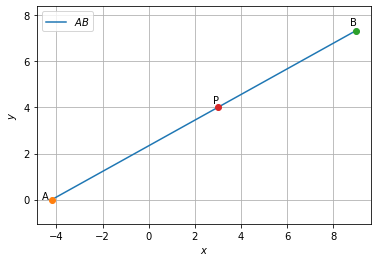
\includegraphics[width=\columnwidth]{solutions/su2021/2/5/Figure4.png}
\caption{Line $AB$}
\label{su2021/2/5/fig:line}	
\end{figure}



